%ch.tex


\chapter{Zippers and contexts and URI's, oh my!}
\begin{center}
{\small\em Zippers are not just for Bruno anymore}
\end{center}

\section{Zippers are not just for Bruno anymore}

\subsection{The history of the zipper}

The origin of the zipper rests in the desire to provide an efficient
functional representation of a ``structure'' editor. For example, we
might consider navigation and destructive modification of a tree. In a
functional representation destructive operations need to be replaced
by copying. Done naively, this can be very expensive.

\subsubsection{Huet's zipper}

In his functional pearl Huet describes a generic approach to the
problem of an applicative structure editor. He dubbed it the
zipper. The key idea is to denote the location of a position in a tree
by splitting it into two pieces: the subtree of focus and the context
in which it appears.

To render this idea in \texttt{Scala} suppose that we have modeled the
type of a tree as

\begin{lstlisting}[language=Scala,mathescape=true]
  trait Tree[A]
  // Leaf
  class TreeItem[A]( val item : A ) extends Tree[A]
  // Branches
  class TreeSection[A](
    val section: List[Tree[A]]
  ) extends Tree[A]  
\end{lstlisting}

with corresponding companion objects for easy construction and
deconstruction. (We'd make these
\lstinline[language=Scala,mathescape=true]!case class!es, but then we
couldn't use inheritance.)

\begin{lstlisting}[language=Scala,mathescape=true]
  object TreeItem {
    def apply[A]( item : A ) = { new TreeItem( item ) }
    def unapply[A]( tree : TreeItem[A] )
    : Option[( A )] = {
      Some( ( tree.item ) )
    }
  }
  object TreeSection {
    def apply[A]( section : List[Tree[A]] ) = {
      new TreeSection( section )
    }
    def unapply[A]( tree : TreeSection[A] )
    : Option[( List[Tree[A]] )] = {
      Some( ( tree.section ) )
    }
  }
\end{lstlisting}

then we would model a context in the tree as

\begin{lstlisting}[language=Scala,mathescape=true]
  trait Context[A]
  case class Top[A]( ) extends Context[A]
  class TreeContext[A](
    val left : List[Tree[A]],
    val ctxt : Context[A],
    val right : List[Tree[A]]
  ) extends Context[A]
\end{lstlisting}

Essentially, a \lstinline[language=Scala,mathescape=true]!Context!
denotes a place where we might ``plugin'' a subtree. Thus, it
identifies the branches to the left, the branches to the right and a
``path'' to a ``hole''.

Of course, we have the obligatory companion object.

\begin{lstlisting}[language=Scala,mathescape=true]
  object TreeContext {
    def apply[A](
      left : List[Tree[A]],
      ctxt : Context[A],
      right : List[Tree[A]] ) = {
        new TreeContext( left, ctxt, right )
      }
      def unapply[A]( ctxt : TreeContext[A] )
      : Option[( List[Tree[A]], Context[A], List[Tree[A]] )] = {
        Some( ( ctxt.left, ctxt.ctxt, ctxt.right ) )
      }
  }
\end{lstlisting}

Since it is clear how this boilerplate is made, we will dispense with
it in subsequent discussion; but note that the cost in boilerplate may
not have been worth deprecating inheritance in
\lstinline[language=Scala,mathescape=true]!case class!es.

Now, we have the types necessary to model our intuitions as to what a
location is. It's a pair of a context and a tree that plugs into the
context. Note that neither of these datum are suffient in an of
themselves to identify a location in a tree. The subtree could occur
in any number of trees. Likewise, the context could be filled with any
number of subtrees. It takes the pair to identify a location in a
tree. For those with some experience in mathematics, this idea is
strongly reminiscent of both Dedekind cuts and Conway's models of
games as numbers.

\begin{lstlisting}[language=Scala,mathescape=true]
  class Location[A](
    val tree : Tree[A],
    val ctxt : Context[A]
  )  
\end{lstlisting}

As a paradigmatic example consider (a crude model of) the syntax tree
of an arithmetic expression. (Now, the decision to model a tree as a
\lstinline[language=Scala,mathescape=true]!class! becomes clear.)

\begin{lstlisting}[language=Scala,mathescape=true]
  case class Token[A](
   override item : A
  ) extends TreeItem[A]( item )
  case class AST[A](
    override section : List[Tree[A]]
  ) extends TreeSection[A]( section )
\end{lstlisting}

Then an instance might look like

\begin{lstlisting}[language=Scala,mathescape=true]
  AST[String](
    List(
      AST[String](
        List(
          Token[String]( "a" ),
          Token[String]( "*" ),
          Token[String]( "b" )
        )
      ),
      Token[String]( "+" ),
      AST[String](
        List(
          Token[String]( "c" ),
          Token[String]( "*" ),
          Token[String]( "d" )
        )
      )
    )
  )
\end{lstlisting}

Then the location of the second multiplication sign is:

\begin{lstlisting}[language=Scala,mathescape=true]
  Location[String](
    Token[String]( "*" ),
    TreeContext[String](
      List( Token[String]( "c" ) ),
      TreeContext[String](
        List(
          Token[String]( "+" ),
          AST[String](
            List(
              Token[String]( "a" ),
              Token[String]( "*" ),
              Token[String]( "b" )
              )
            )
          ),
          Top( ),
          List( )
          ),
      List( Token[String]( "d" ) )
    )
  )
\end{lstlisting}

\paragraph{The navigation functions} With this structure we can define
generic navigation functions.

\begin{lstlisting}[language=Scala,mathescape=true]
trait ZipperNavigation[A] {
  def left( location : Location[A] ) : Location[A] = {
    location match {
      case Location( _, Top ) => {
        throw new Exception( "left of top" )
      }
      case Location( t, TreeContext( l :: left, up, right ) ) => {
        Location( l, TreeContext( left, up, t :: right ) )
      }
      case Location( t, TreeContext( Nil, up, right ) ) => {
        throw new Exception( "left of first" )
      }
    }
  }
  def right( location : Location[A] ) : Location[A] = {
    location match {
      case Location( _, Top ) => {
        throw new Exception( "right of top" )
      }
      case Location( t, TreeContext( left, up, r :: right ) ) => {
        Location( r, TreeContext( t :: left, up, right ) )
      }
      case Location( t, _ ) => {
        throw new Exception( "right of last" )
      }
    }
  }
  def up( location : Location[A] ) : Location[A] = {
    location match {
      case Location( _, Top ) => {
        throw new Exception( "up of top" )
      }   
      case Location( t, TreeContext( left, up, right ) ) => {
        Location( TreeSection[A]( left.reverse ::: ( t :: right ) ),
                  up )
      }
    }
  }
  def down( location : Location[A] ) : Location[A] = {
    location match {
      case Location( TreeItem( _ ), _ ) => {
        throw new Exception( "down of item" )
      }
      case Location( TreeSection( u :: trees ), ctxt ) => {
        Location( u, Context( Nil, ctxt, trees ) )
      }
    }
  }
}
\end{lstlisting}

\paragraph{Exercising the zipper} We can exercise the zipper
navigation functions using the two examples from above.

\begin{lstlisting}[language=Scala,mathescape=true]
  object Exercise extends ZipperNavigation[String] {
    val arithmeticExpr1 = ...

    val locationOf2ndMult = ...

     def show( depth : Int )( tree : Tree[String] ) : Unit = {
       tree match {
         case TreeItem( item : String ) => {
           val indent =
           ( "" /: (1 to depth) )( { ( acc, d ) => acc + " " } )
           println( indent + "Leaf : " + item )
         }
         case TreeSection( section : List[Tree[String]] ) => {
           for( t <- section ){ show( depth + 2 )( t ) }
         }
       }
     }     
   }
\end{lstlisting}

\begin{lstlisting}[language=Scala,mathescape=true]
  scala> import Exercise._
  import Exercise._
  import Exercise._

  scala> show( 0 )( arithmeticExpr1 )
  show( 0 )( arithmeticExpr1 )
    Leaf : a
    Leaf : *
    Leaf : b
  Leaf : +
    Leaf : c
    Leaf : *
    Leaf : d

  scala> show( 0 )( locationOf2ndMult.tree )
  show( 0 )( locationOf2ndMult.tree )
  Leaf : *

  scala> show( 0 )( up( locationOf2ndMult ).tree )
  show( 0 )( up( locationOf2ndMult ).tree )
  Leaf : c
  Leaf : *
  Leaf : d

  scala> show( 0 )( up( up( locationOf2ndMult ) ).tree )
  show( 0 )( up( up( locationOf2ndMult ) ).tree )
    Leaf : a
    Leaf : *
    Leaf : b
  Leaf : +
    Leaf : c
    Leaf : *
    Leaf : d

  scala> show( 0 )( up( up( up( locationOf2ndMult ) ) ).tree )
  show( 0 )( up( up( up( locationOf2ndMult ) ) ).tree )
  java.lang.Exception: up of top
        ...
  scala> 
\end{lstlisting}

Of course, the real desiderata are the mutation functions.

\begin{lstlisting}
  trait ZipperMutation[A] {
    def update(
    location : Location[A], tree : Tree[A]
    ) : Location[A] = {
      location match {
        case Location( _, ctxt ) =>
	  Location( tree, ctxt )
        }
      }
    def insertRight(
      location : Location[A], tree : Tree[A]
    ) : Location[A] = {
      location match {
        case Location( _, Top( ) ) => {
          throw new Exception( "insert of top" )
        }
        case Location(
	  curr, TreeContext( left, up, right )
        ) => {
          Location(
	    curr, TreeContext( left, up, tree :: right )
          )	
        }
      }    
    }
    def insertLeft(
      location : Location[A], tree : Tree[A]
    ) : Location[A] = {
      location match {
        case Location( _, Top( ) ) => {
          throw new Exception( "insert of top" )
        }
        case Location(
	  curr, TreeContext( left, up, right )
        ) => {
          Location(
	    curr, TreeContext( tree :: left, up, right )
          )	
        }
      }    
    }
    def insertDown(
      location : Location[A], tree : Tree[A]
    ) : Location[A] = {
      location match {
        case Location( TreeItem( _ ), _ ) => {
          throw new Exception( "down of item" )
        }
        case Location(
	  TreeSection( progeny ), ctxt
        ) => {
          Location(
	    tree, TreeContext( Nil, ctxt, progeny )
          )
        }
      }
    }
    def delete(
      location : Location[A], tree : Tree[A]
    ) : Location[A] = {
      location match {
        case Location( _, Top( ) ) => {
          throw new Exception( "delete of top" )
        }
        case Location(
	  _, TreeContext( left, up, r :: right )
        ) => {
          Location(
	    r, TreeContext( left, up, right )
          )
        }
        case Location(
	  _, TreeContext( l :: left, up, Nil )
        ) => {
          Location(
	    l, TreeContext( left, up, Nil )
          )
        }
        case Location(
	  _, TreeContext( Nil, up, Nil )
        ) => {
          Location( TreeSection( Nil ), up )
        }
      }
    }
  }
\end{lstlisting}

\subsubsection{Zippers generically}


\section{Zipper and one-holed contexts}

\section{Differentiation and contexts}

\subsection{Regular types}

\subsection{Container types}

\section{Generic zipper -- differentiating navigation}

In this section we build a bridge between Oleg Kiselyov's Haskell
implementation of the generic zipper. This is a transliteration of his
original code. As such, we provide a veneer over \texttt{Scala}'s
native delimited continuation library. Then we use this veneer to
express a direct translation of Oleg's code.

\begin{lstlisting}[language=Scala,mathescape=true]
  object MonadDefns {
    type MonadLike = { 
      def map[A,B]( f : A => B )
      def flatMap[M[_],A,B]( f : A => M[B] )
      def filter[A]( p : A => Boolean )
      def lift[ML[_],MU[_],A]( m : ML[A] ) : MU[A]
    }
  }

  trait StateT[V,M[_],A]{
  }

  trait CC[R,M[_],A] {
    def k2P : K[R,M,A,_] => StateT[Int,M,A]
  }

  trait Prompt[R,A] {
  }

  trait Frame[M[_],R,A,B]{
    def a2CC : A => CC[R,M,B]
  }

  trait K[R,M[_],A,B]{
    def frame : Frame[M,R,A,B]
    def r : R
    def a : A
    def b : B

    def map[C]( f : A => C )
    def flatMap[C]( f : A => K[R,M,A,C] )
    def filter( p : A => Boolean )
    def lift( m : M[A] ) : CC[R,M,A]
  }

  trait SubK[R,M[_],A,B] extends K[R,M,A,B]{
  }

  trait ControlOps[R,M[_],A] {
    def appk[B]( k : K[R,M,A,B], a : A ) : StateT[Int,M,A]
    def runCC( cc : CC[R,M,A] ) : M[A]
    def promptP( f : Prompt[R,A] => CC[R,M,A] ) : CC[R,M,A]
    def shiftP[B](
      p : Prompt[R,B],
      f : (CC[R,M,A] => CC[R,M,B]) => CC[R,M,B]
    ) : CC[R,M,A]
}
\end{lstlisting}

Essentially, a zipper in this new style wraps a term. It may also
contain a traversal function.

\begin{lstlisting}[language=Scala,mathescape=true]  
  trait Zipper[R,M[_],T,D] {
    def term : T
  }

  class DCZipper[R,M[_],T,D](
    override val term : T,
    val traversal : CC[R,M,(Option[T],D)] => CC[R,M,Zipper[R,M,T,D]]
  ) extends Zipper[R,M,T,D]

  class ZipDone[R,M[_],T,D](
    override val term : T
  ) extends Zipper[R,M,T,D]
\end{lstlisting}

\break

We then provide basic factory mechanism for constructing zippers and
then using them.

\begin{lstlisting}[language=Scala,mathescape=true]
  trait ZipperOps[R,M[_],T,D] {
    def zipTerm(
      traversal
      : ( ( T => CC[R,M,( Option[T], D )] ), T )
        => CC[R,M,T],
      term : T
    ) : CC[R,M,Zipper[R,M,T,D]]
    def zipThrough( zipper : Zipper[R,M,T,D] ) : Unit
  }
\end{lstlisting}

\subsection{Delimited continuations}

\section{Species of Structure}
\section{Constructing contexts and zippers from data types}

The key intuition is that a zipper is a ``focus'' on a subterm of a
term. The data needed to capture this idea is a pair,
\lstinline[language=Scala,mathescape=true]!(T,$\partial$)!, the
subterm itself, and the context in which it occurs. Using types to
guide our intuition we see that the subterm must have the same type as
a term while the type of a context is determined by a calculation that
perfectly matches a version of the derivative one might have learned
in high school calculus -- but applied to data structures.

\subsection{Contexts}

\begin{figure}[tbp]
\begin{center}
{ 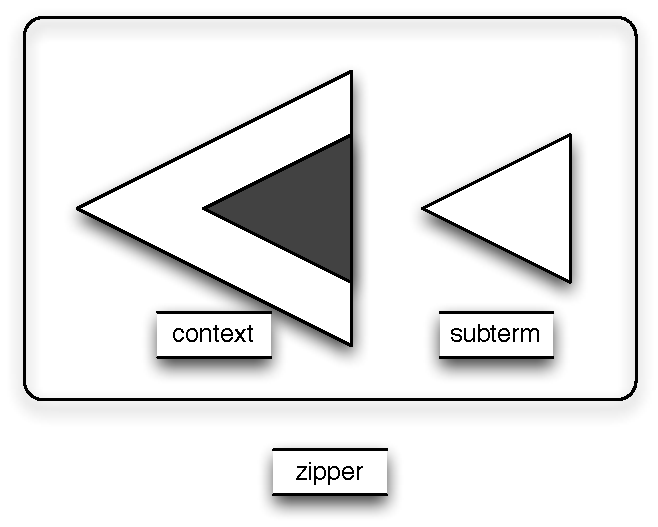
\includegraphics[scale=.65]{/Users/lgm/work/src/projex/biosimilarity/trace/src/main/book/content/figures/ZipperContext1.pdf} }
\caption{ Context and subterm }
\end{center}
\end{figure}

\begin{mathpar}
  \inferrule* {} {\partial Const_A = 0}
  \\
  \inferrule* {} {\partial Id = 0}
  \\
  \inferrule* {} {\partial F + G = \partial F + \partial G}
  \\
  \inferrule* {} {\partial F \times G = F \times \partial G + \partial F \times G}
  \\
  \inferrule* {} {\partial F \circ G = \partial F \circ G \times G}
\end{mathpar}

\begin{figure}[tbp]
\begin{center}
{ 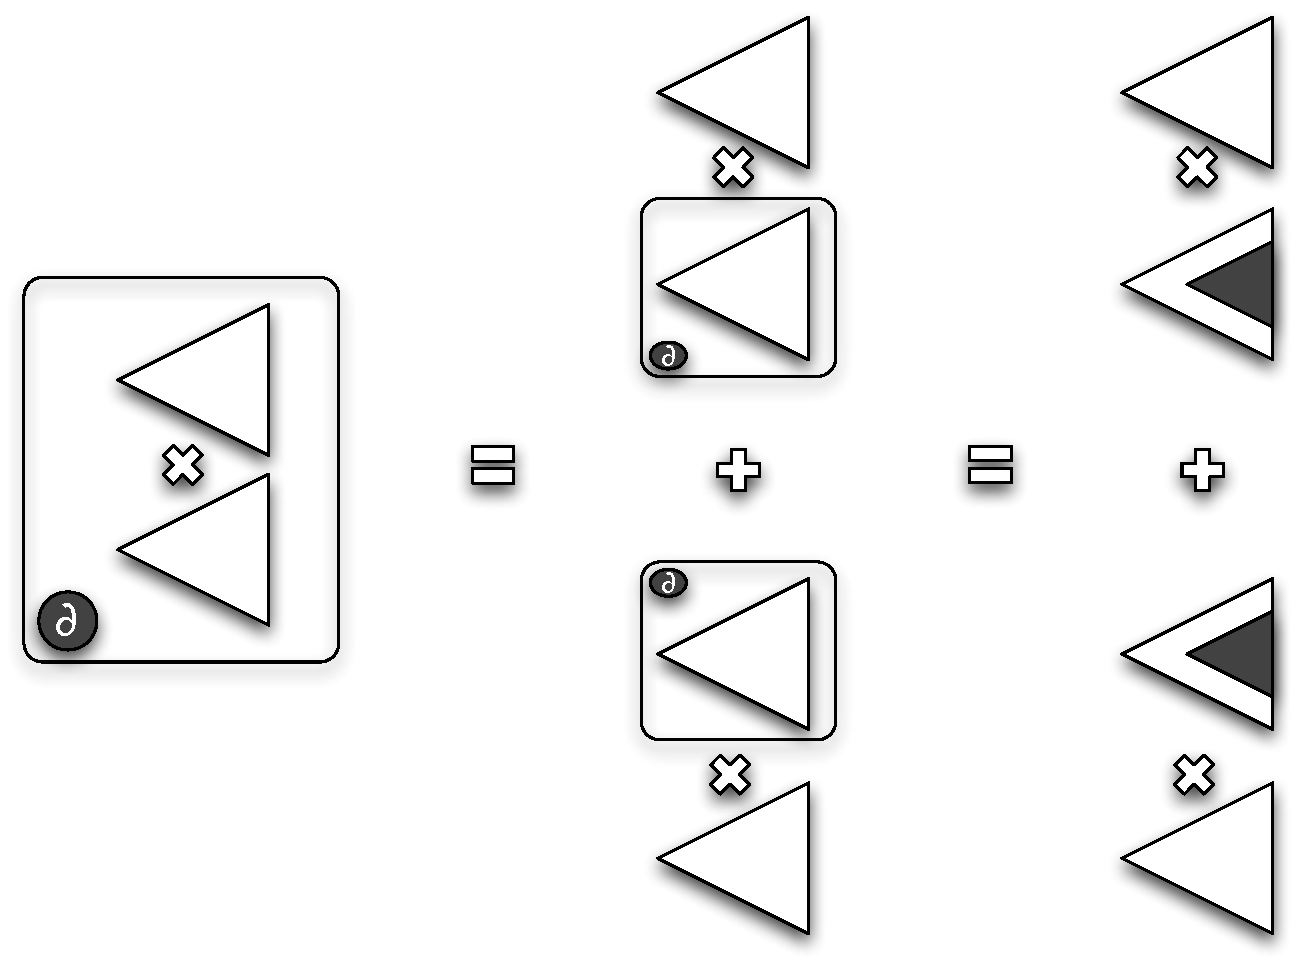
\includegraphics[scale=.75]{/Users/lgm/work/src/projex/biosimilarity/trace/src/main/book/content/figures/Derivative.pdf} }
\caption{ Context and subterm }
\end{center}
\end{figure}

\subsection{Zippers}

\begin{lstlisting}[language=Scala]
  case class Context[Name, NSeq <: NmSeq[Name]](
     override val self : RegularType[Name,NSeq]
  )
  extends RegularType[Name, NSeq] with Proxy {
    override def support = self.support
  }

  trait Contextual[Name, NSeq <: NmSeq[Name]]
  extends Differential[Name,NSeq]  {
    def holePunch( support : NSeq )(
       x : Name, regularType : RegularType[Name,NSeq]
    ) : Context[Name,NSeq] = {
      fresh match {
        case None => throw new Exception( "out of names" )
        case Some( cX ) => {
          val fixRT =
	  RegularFixPt[Name,NSeq](
             (fresh match {
               case None =>
                  throw new Exception( "out of names" )
               case Some( fX ) => fX
             }),
             regularType,
             support
          )
          Context[Name,NSeq](
	     RegularFixPt[Name,NSeq](
                cX,
             RegularSum[Name,NSeq](
                List(
		   RegularUnity[Name,NSeq]( support ),
                   RegularProduct[Name,NSeq](
                      List(
                         RegularFPEnv[Name,NSeq](
                         x,
                         partial( x, regularType ),
                         fixRT,
                         support
		         ),
                         RegularMention[Name,NSeq](
                            cX,
                            support
                         )
		      ),
                      support
                   )
                ),
                support
             ),
             support
           )
        )
      }
    }
  }
}
\end{lstlisting}

\begin{lstlisting}[language=Scala,mathescape=true]
  trait Differential[Name, NSeq <: NmSeq[Name]] 
  extends NmSeqOps[Name,NSeq] {
    def regularNull( supp : NSeq ) : RegularNullity[Name,NSeq]
    def regularUnit( supp : NSeq ) : RegularUnity[Name,NSeq]
    def partial( x : Name, rtype : RegularType[Name, NSeq] )
    : RegularType[Name, NSeq] = {
      rtype match {
        case RegularMention( y, supp ) => {
          if ( x == y ) {
            regularUnit( supp )
          }
          else {
            regularNull( supp )
          }
        }
        case RegularNullity( supp ) => regularNull( supp )
        case RegularUnity( supp ) => regularNull( supp )
        case RegularSum( s, supp ) => {
          RegularSum(
	     s.map(
               {
                 ( rt : RegularType[Name,NSeq]) => {
                   partial( x, rt )
                 }
               }
             ),
             supp
          )
        }
        case RegularProduct( s, supp ) => {
          val right = s.dropRight( 1 )
          RegularSum[Name,NSeq](
	     List(
                RegularProduct[Name,NSeq](
                   List(
                      partial( x, s( 0 ) ),
                      RegularProduct[Name,NSeq](
                         right,
                         supp
                      )
                   ),
                   supp
                ),
                RegularProduct[Name,NSeq](
                   List(
                      s( 0 ),
                      partial(
                         x,
                         RegularProduct[Name,NSeq]( right, supp )
                      )
                   ),
                   supp
                )
	     ),
             supp
	  )
        }
        case RegularFixPt( v, e, supp ) => {
          val z = fresh match {
            case None => throw new Exception( "out of names" )
            case Some( fn ) => fn
          }
          RegularSum[Name,NSeq](
	     List( 
                RegularFixPt(
                   z, 
                   partial(
		      x,
                      RegularWeakening(
                         z,
                         RegularFPEnv( v, e, rtype, supp ),
                         supp
                      )
                   ),
                   supp
                ),
                RegularProduct(
                   List(
                      partial(
                         v,
                         RegularFPEnv(
                            v,
                            e,
                            rtype,
                            supp
		         )
                      ),
                      RegularMention( z, supp )
                   ),
                   supp
                )
             ),
             supp
	   )
         }
         case RegularFPEnv( v, e, s, supp ) => {
           RegularSum(
              List(
                 RegularFPEnv(
                    v,
                    partial( x, e ),
                    s,
                    supp
                 ),
                 // BUGBUG -- lgm -- have i got the association correct
                 RegularProduct(
                    List(
                       RegularFPEnv(
                          v,
                          partial( v, e ),
                          s,
                          supp
                       ),
                       partial( x, s )
                    ),
                    supp
                 )
              ),
              supp
           )
         }
         case RegularWeakening( v, e, supp ) => {
           if ( x == v ) {
             regularNull( supp )
           }
           else {
             RegularWeakening( v, partial( x, e ), supp )
           }
         }
       }
     }
   }
\end{lstlisting}
\section{Mapping URIs to zipper-based paths and back}

\subsection{Path and context}

\subsection{Homomorphisms and obfuscation}

\section{Applying zippers to our project}

\begin{figure}[tbp]
\begin{center}
{ 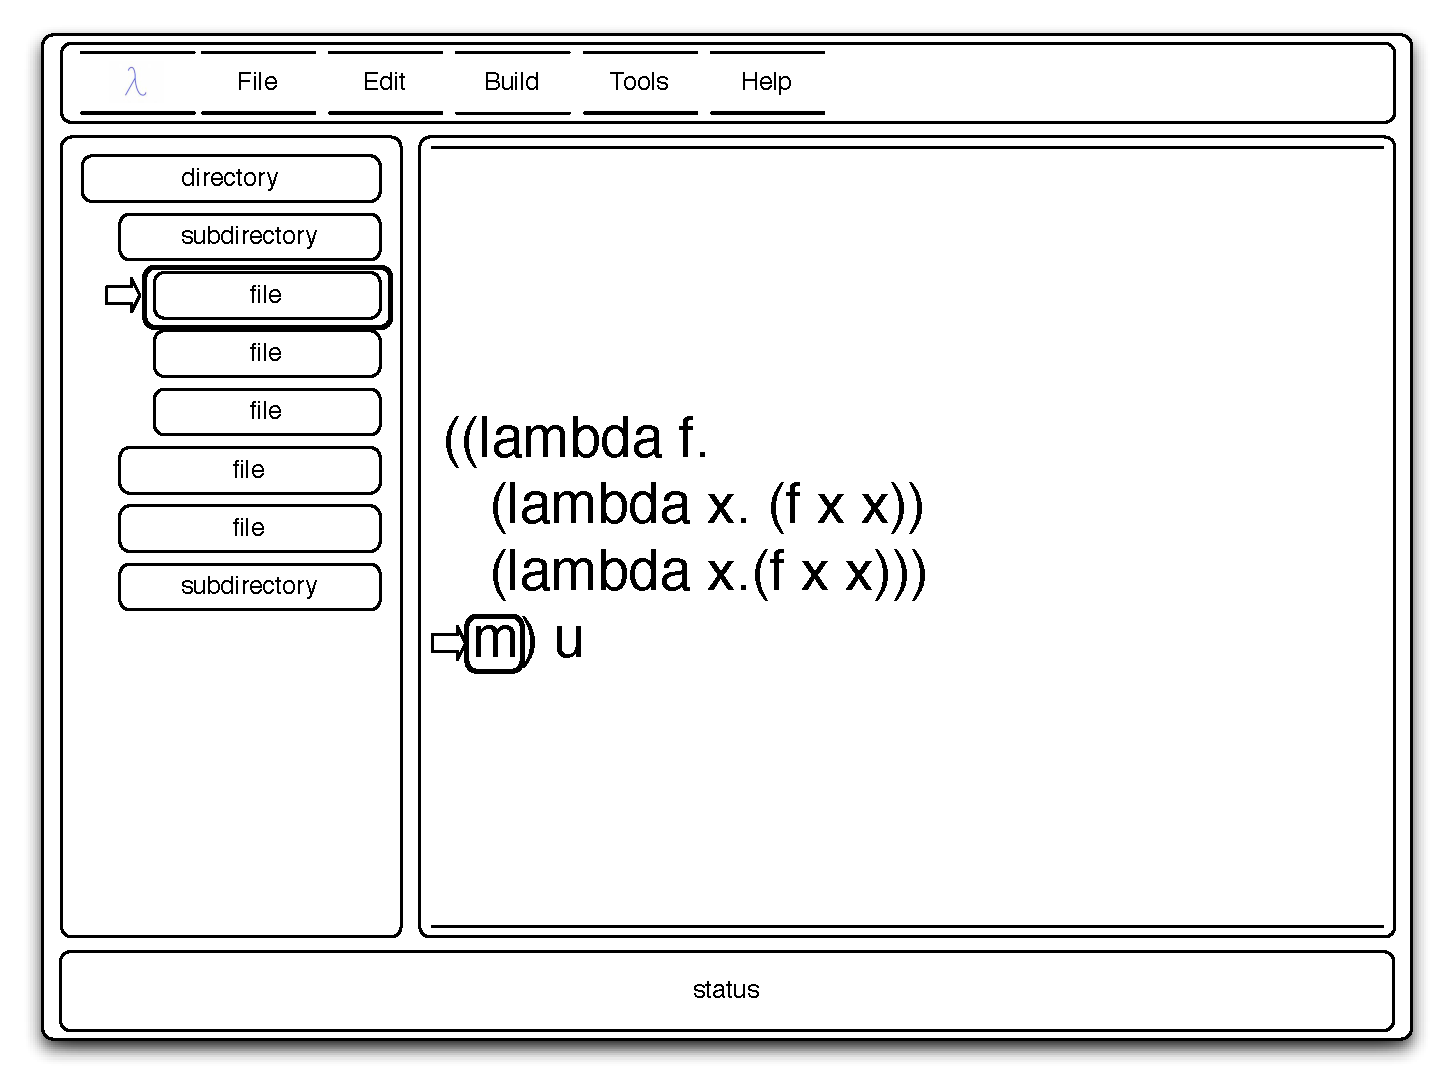
\includegraphics[scale=.65]{/Users/lgm/work/src/projex/biosimilarity/trace/src/main/book/content/figures/ProjectZipper.pdf} }
\caption{ Zippers and editors }
\end{center}
\end{figure}
\subsection{Navigating and editing terms}

Consider the following term.

\begin{lstlisting}[language=Scala,mathescape=true]
  // Corresponds to the Church numeral: 
  // $\lambda \; f . \; \lambda \; x . $
  //     $(f \; \lambda \; f . \; f \; \lambda \; f \; . \; \lambda \; x . \; x )$
  //     $((f \; \lambda \; f \; . \; \lambda \; x . \; x) x)$ 
  Abstraction(
    List( StringLiteral( "f" ) ),
    Abstraction(
      List( StringLiteral( "x" ) ),
      Application( 
        Application(
          Mention( StringLiteral( "f" ) ),
          Abstraction( 
            List( StringLiteral( "f" ) ),
            Application( 
              Mention( StringLiteral( "f" ) ),
              Abstraction(
                List( StringLiteral( "f" ) ),
                Abstraction(
                  List( StringLiteral( "x" ) ),
                  Mention( StringLiteral( "x" ) )
                )
              )
            )
          )
        ),
        Application(
          Application( 
            Mention( StringLiteral( "f" ) ),
            Abstraction(
              List( StringLiteral( "f" ) ),
              Abstraction(
                List( StringLiteral( "x" ) ),
                Mention( StringLiteral( "x" ) )
              )
            )
          ),
          Mention( StringLiteral( "x" ) )  
        )
      )
    )
  )
\end{lstlisting}

\subsection{Navigating and editing projects}


% \section{Existence problems}
% We begin with some metamathematics.
% All problems about the existence of maps can be cast into one of the
% following two forms, which are in a sense mutually dual.

% \noindent
% {\bf The Extension Problem}\index{extension problem} \    %%% NB index entry tag
% Given an inclusion $ A \stackrel{i}{\hookrightarrow} X $, and a map
% $ A \stackrel{f}{\rightarrow} Y $,
% does there exist a map $f^{\dagger}:X\to Y$ such that
% $f^{\dagger}$ agrees with $f$ on $A$?

% Here the appropriate source category for maps should be clear from the
% context and, moreover, commutativity through a
% candidate $f^{\dagger}$ is precisely
% the restriction requirement; that is,
% $$f^{\dagger}   :  f^{\dagger}\circ i = f^{\dagger}|_A = f\,. $$
% If such an $f^{\dagger}$ exists\footnote{${}^{\dagger}$ suggests striving
% for perfection, crusading}, then it is called an {\bf
% extension}\index{extension!of a map|bi} of $f$ and is said to {\bf
% extend}\index{extend|bi} $f$. In any diagrams, the presence of
% a dotted arrow or an arrow carrying a ? indicates a pious hope, in no way
% begging the question of its existence. Note that we shall usually
% omit $\circ$ from composite maps.

% \noindent
% {\bf The Lifting Problem}\index{lifting problem} \
% Given a pair of maps $E \stackrel{p}{\rightarrow}B$ and $X \stackrel{f}
% {\rightarrow} B $,
% does there exist a map $f^{\circ} : X \to E$, with
% $pf^{\circ} = f  $?


% That {\em all\/} existence problems about maps are essentially of one
% type or
% the other from these two is seen as follows. Evidently, all existence problems
% are representable by triangular diagrams\index{triangular diagrams} and it
% is easily seen that there are only these six possibilities:
% \begin{center}\begin{picture}(300,70)  %augch2 75
% \put(5,60){\vector(1,0){30}}
% \put(55,60){\vector(1,0){30}}
% \put(135,60){\vector(-1,0){30}}
% \put(185,60){\vector(-1,0){30}}
% \put(235,60){\vector(-1,0){30}}
% \put(285,60){\vector(-1,0){30}}
% \put(0,55){\vector(0,-1){30}}
% \put(50,55){\vector(0,-1){30}}
% \put(100,25){\vector(0,1){30}}
% \put(150,25){\vector(0,1){30}}
% \put(200,55){\vector(0,-1){30}}
% \put(250,55){\vector(0,-1){30}}
% \put(28,33){\small ?}
% \put(78,33){\small ?}
% \put(128,33){\small ?}
% \put(178,33){\small ?}
% \put(228,33){\small ?}
% \put(278,33){\small ?}
% \put(10,3){\bf 1}
% \put(60,3){\bf 2}
% \put(110,3){\bf 3}
% \put(160,3){\bf 4}
% \put(210,3){\bf 5}
% \put(260,3){\bf 6}
% \put(35,55){\vector(-1,-1){30}}
% \put(155,25){\vector(1,1){30}}
% \put(135,55){\vector(-1,-1){30}}
% \put(55,25){\vector(1,1){30}}
% \put(235,55){\vector(-1,-1){30}}
% \put(255,25){\vector(1,1){30}}
% \end{picture}\end{center}



% \begin{figure}
% \begin{picture}(300,220)(0,0)
% \put(-20,-20){\resizebox{20 cm}{!}{\includegraphics{3dpdf}}}
% \put(260,-10){\resizebox{15 cm}{!}{\includegraphics{contpdf}}}
% \put(220,80){$\beta$}
% \put(400,-10){$N$}
% \put(260,170){$\beta$}
% \put(90,15){$N$}
% \end{picture}
% \caption{{\em The log-gamma family of densities with central mean
% $<N> \, = \frac{1}{2}$ as a surface and as a contour plot. }}
% \label{pdf}
% \end{figure}

\newpage
